\documentclass{standalone}
\usepackage{tikz}

\begin{document}

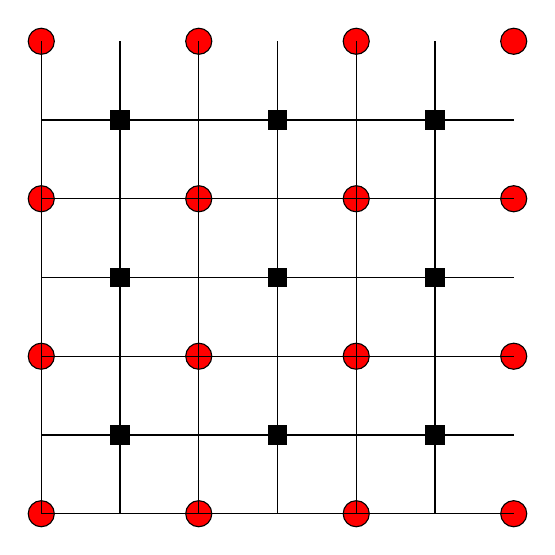
\begin{tikzpicture}[scale=2]

% Define coordinates for the vertices of the square grid
\foreach \x in {0, 1, 2, 3} {
    \foreach \y in {0, 1, 2, 3} {
        \node[draw, circle, fill=red] at (\x, \y) {};
    }
}

% Draw lines between adjacent nodes to form the grid
\foreach \x in {0, 1, 2} {
    \draw (\x, 0) -- (\x, 3);
    \draw (0, \x) -- (3, \x);
}

% Add additional squares to extend the feasible set to size three
\foreach \x in {0, 1, 2} {
    \foreach \y in {0, 1, 2} {
        \node[draw, rectangle, fill=black] at (\x + 0.5, \y + 0.5) {};
    }
}

% Draw lines between adjacent nodes to form the extended grid
\foreach \x in {0, 1, 2} {
    \draw (\x + 0.5, 0) -- (\x + 0.5, 3);
    \draw (0, \x + 0.5) -- (3, \x + 0.5);
}

\end{tikzpicture}

\end{document}